% Overleaf: compile with pdfLaTeX (the default compiler).
% Put this file at the Overleaf project root and upload the images/ folder beside it.
% From Docs/report/, the same figures are also found at ../../images/.
\documentclass[10pt]{article}

\usepackage[margin=1in]{geometry}
\usepackage{booktabs}
\usepackage{amsmath}
\usepackage{graphicx}
\graphicspath{{images/}{../../images/}}
\usepackage[font=small,skip=2pt]{caption}
\usepackage[hidelinks]{hyperref}

\newcommand{\placefig}[1]{%
  \par\vspace{0.4em}%
  \noindent\begin{minipage}{\textwidth}%
  \centering
  #1%
  \end{minipage}%
  \par\vspace{0.5em}%
}

\title{5228 progress report}
\date{September 2026}

\begin{document}
\maketitle

\section{Auxiliary features: construction, limits, and planned checks}
\label{sec:auxiliary}

The prediction target is \texttt{MONTHLY\_RENT}.
The rental row already has the approval month, town, block, street, flat type, flat model, floor area, furnished flag, lease year, and upfront fee.
The auxiliary files (blocks, MRT stations, schools, malls, COE prices, and stocks) do not share that row key.
Nothing below has been screened by correlation with rent, and no model has been trained.
The figures only describe the constructed columns.

\subsection{Rebuild and complete attribute audit}
\label{sec:rebuild}

This part independently reconstructs features from the original rental inputs and every field in all six supplied auxiliary files. The response is monthly rent in SGD.

The source ledger contains 63 input-field positions: ten original rental fields and 53 auxiliary fields. The target is recorded separately. FURNISHED and FEE are explicitly ignored because they only have one value, including derived indicators and interactions; 61 source positions remain for predictors, construction, joins or metadata. Source names, URLs and keys receive explicit roles rather than being labelled causal rent factors.

There are 1,878 conceptual candidates across the recorded families, including 1,595 month-panel candidates. The compact rental table stores 492 candidate columns plus row, month, target and provenance metadata. Individual-stock and adjusted-price candidates remain in the monthly panel and are reduced using training-month preprocessing; this avoids copying the same macro vector onto every rental. The family ledger is a candidate universe, not the fitted model dimension.

\begin{center}
\small
\begin{tabular}{lr}
\toprule
Candidate family & Columns \\
\midrule
Block structure & 5 \\
Location & 11 \\
MRT & 122 \\
Schools & 123 \\
Malls & 8 \\
COE & 164 \\
Stocks & 1200 \\
Adjusted-price sensitivity & 231 \\
Original & 14 \\
\bottomrule
\end{tabular}
\end{center}

\paragraph{Construction and limitations.}
The normalized town/block/street key is checked as a many-to-one link, with rental row identity and order preserved. Block features retain latitude, longitude, postal and geographic labels, completion year and maximum building floor; ages, density and location summaries are derived. The maximum floor is not the unit floor. MRT construction distinguishes code rows from deduplicated entities, open/planned snapshot status, line-code prefixes, interchange descriptors, distances and radius counts. The new open-distance pool is every supplied snapshot-open station entity, potentially including LRT, rather than the narrower trunk-prefix pool described in the preserved historical text. Observed prefixes are not a verified external line taxonomy; station-name and line-count descriptors may combine open/planned codes at one entity and are read only as snapshot descriptions. Schools include observed primary, secondary, JC/CI and mixed-stage definitions, type, gender, session, address and transport-text descriptors. Malls contribute identity, nearest distances and radius counts. COE uses all supplied categories and rounds, with premium, prevailing premium, quota, bids and derived differences/ratios. Stocks audit all 77 symbols and all OHLC, adjusted-close and volume fields. Adjusted-price descriptors are a separately labelled retrospective sensitivity.

\subsection{Distribution, composition and geographic coverage}
Among saved town/flat-type cells with at least 200 rentals, the median range runs from 2000.00 SGD in bukit merah / 2 room (303 records) to 4650.00 SGD in central / 5 room (200 records). These are composition-specific descriptive medians, not adjusted location effects.

\placefig{%
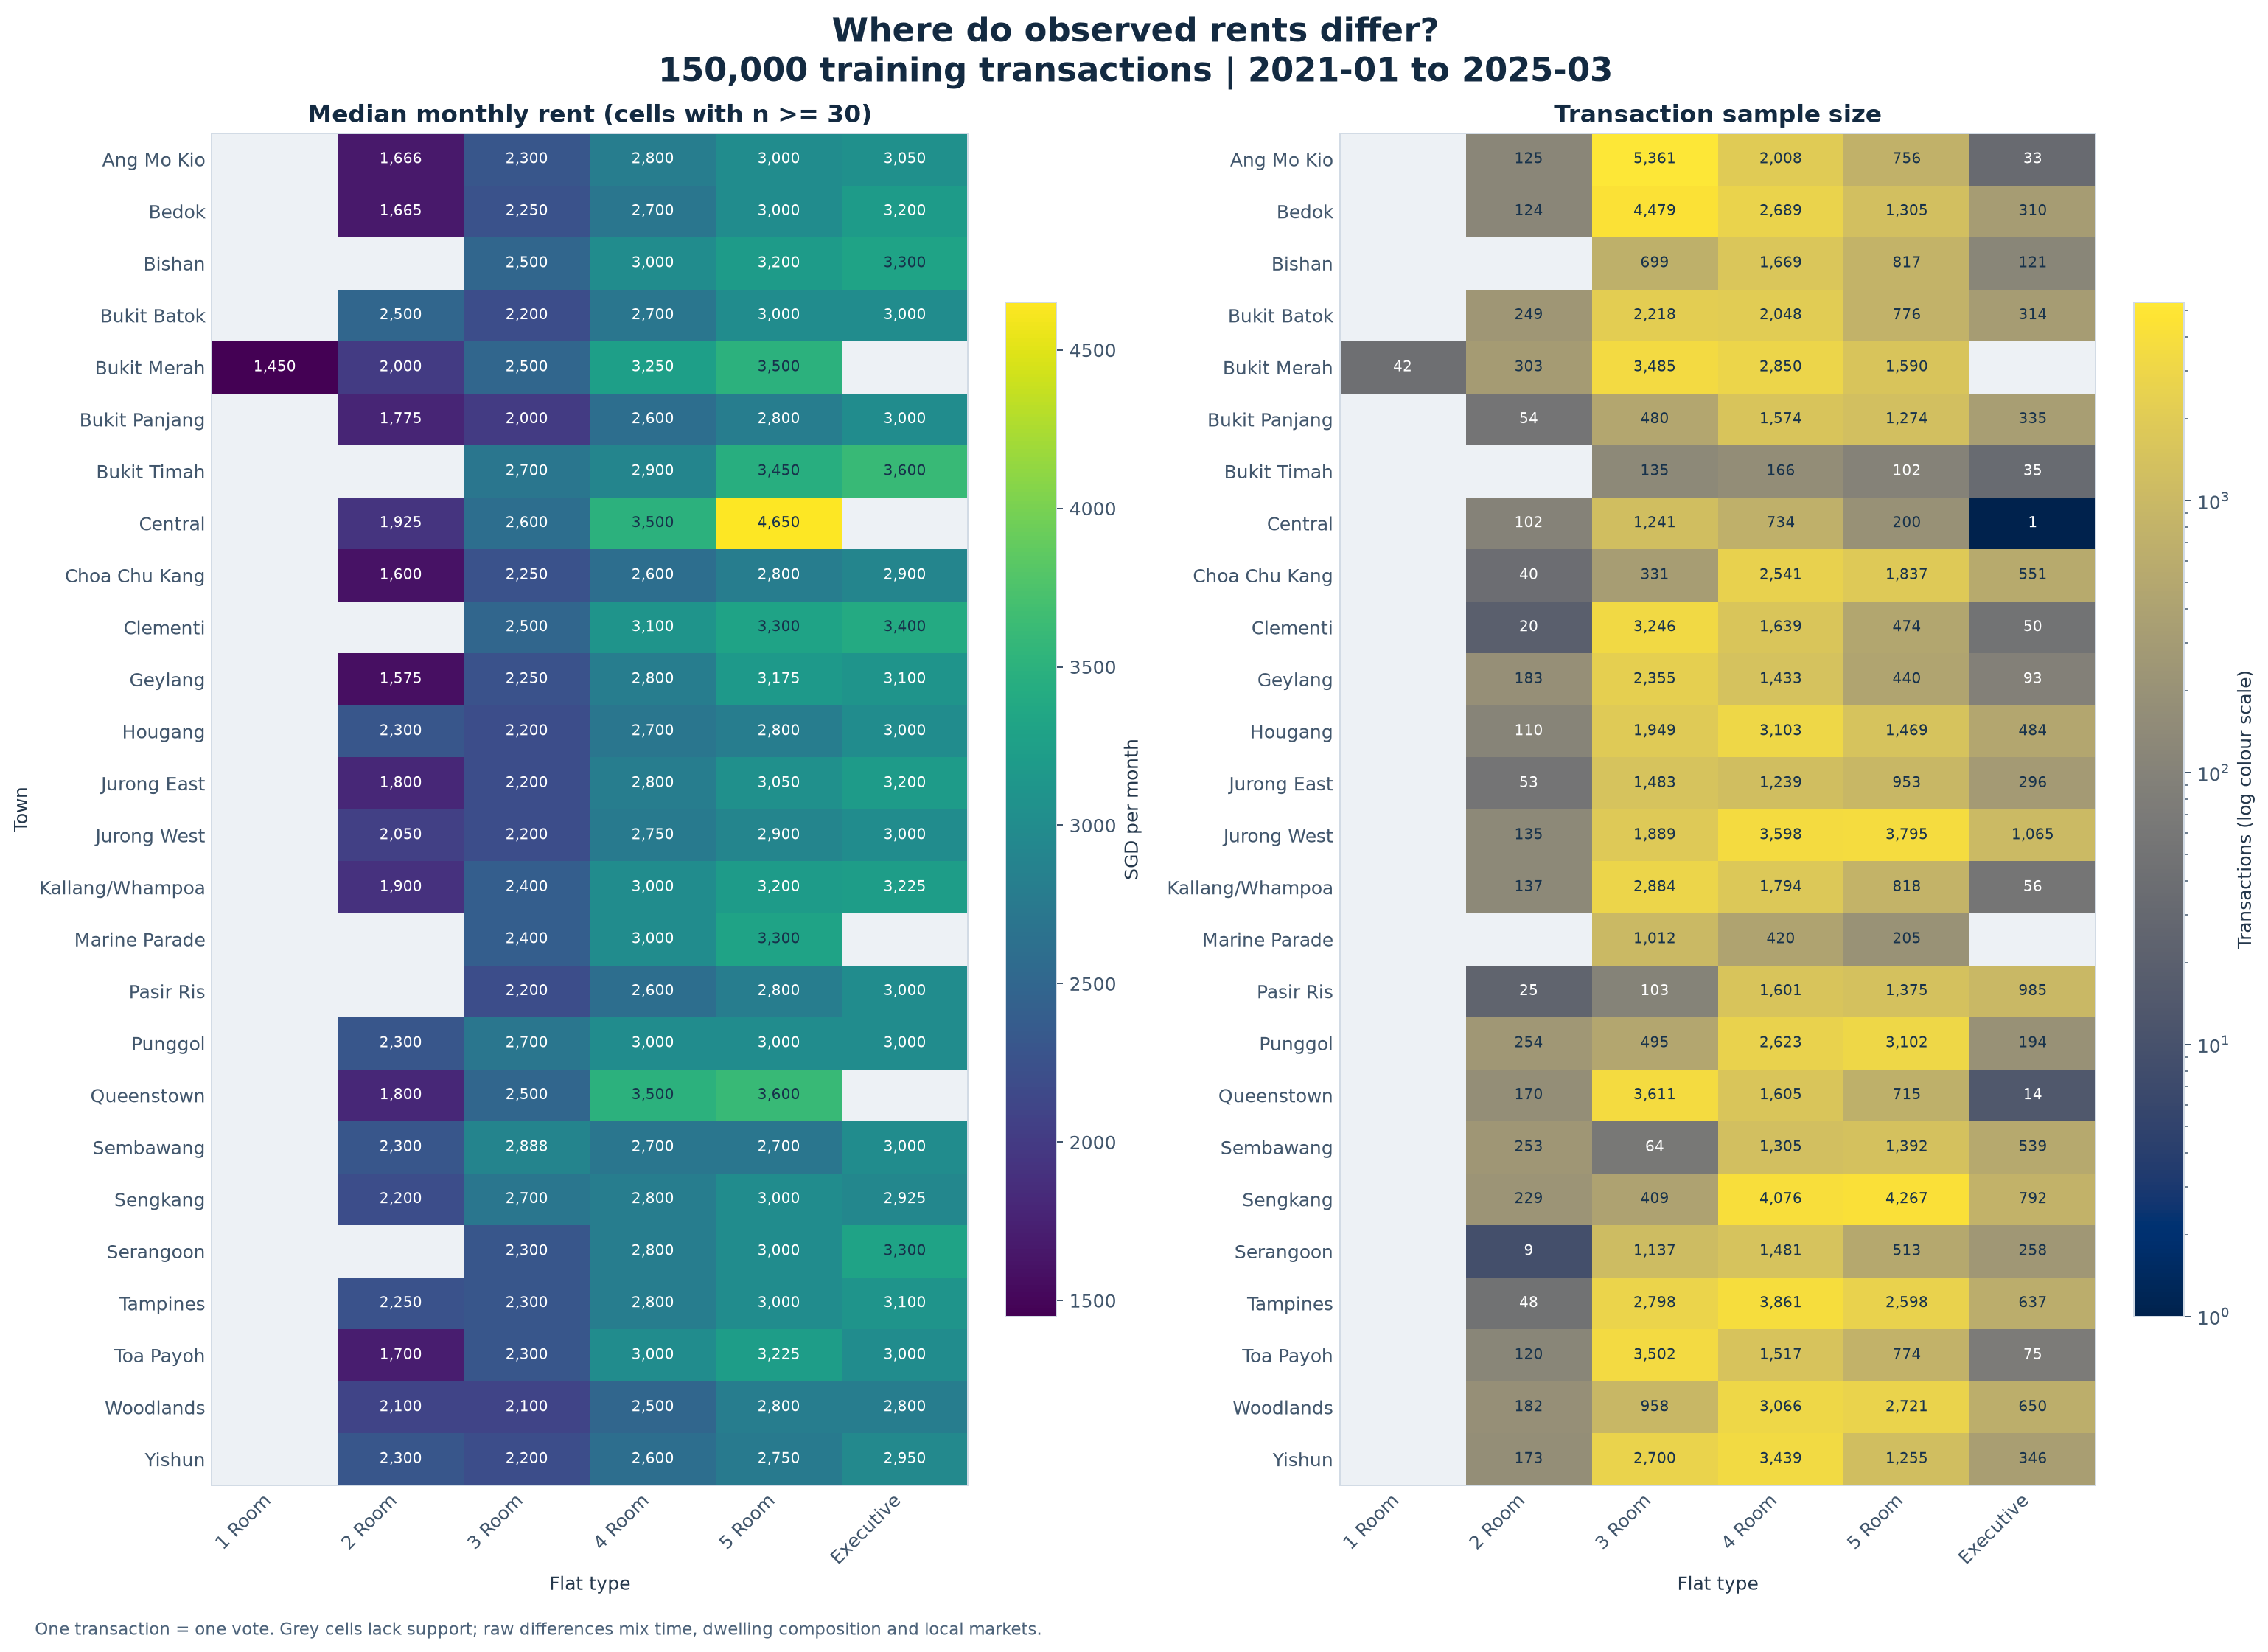
\includegraphics[width=0.96\linewidth,height=0.78\textheight,keepaspectratio]{images/distribution_01_town_flat.png}
\\[0.35em]
\refstepcounter{figure}%
{\small Figure~\thefigure: Town by flat type: median observed rent and sample count.}%
\label{fig:rebuiltdistributiontown}%
}

The time-by-town display contrasts raw monthly median rent with mean rent residual after a full-training Ridge composition fit using area, log area, flat type, flat model and town, without month controls. The residual is observed minus fitted rent, in SGD, and is descriptive rather than out-of-sample error.

\placefig{%
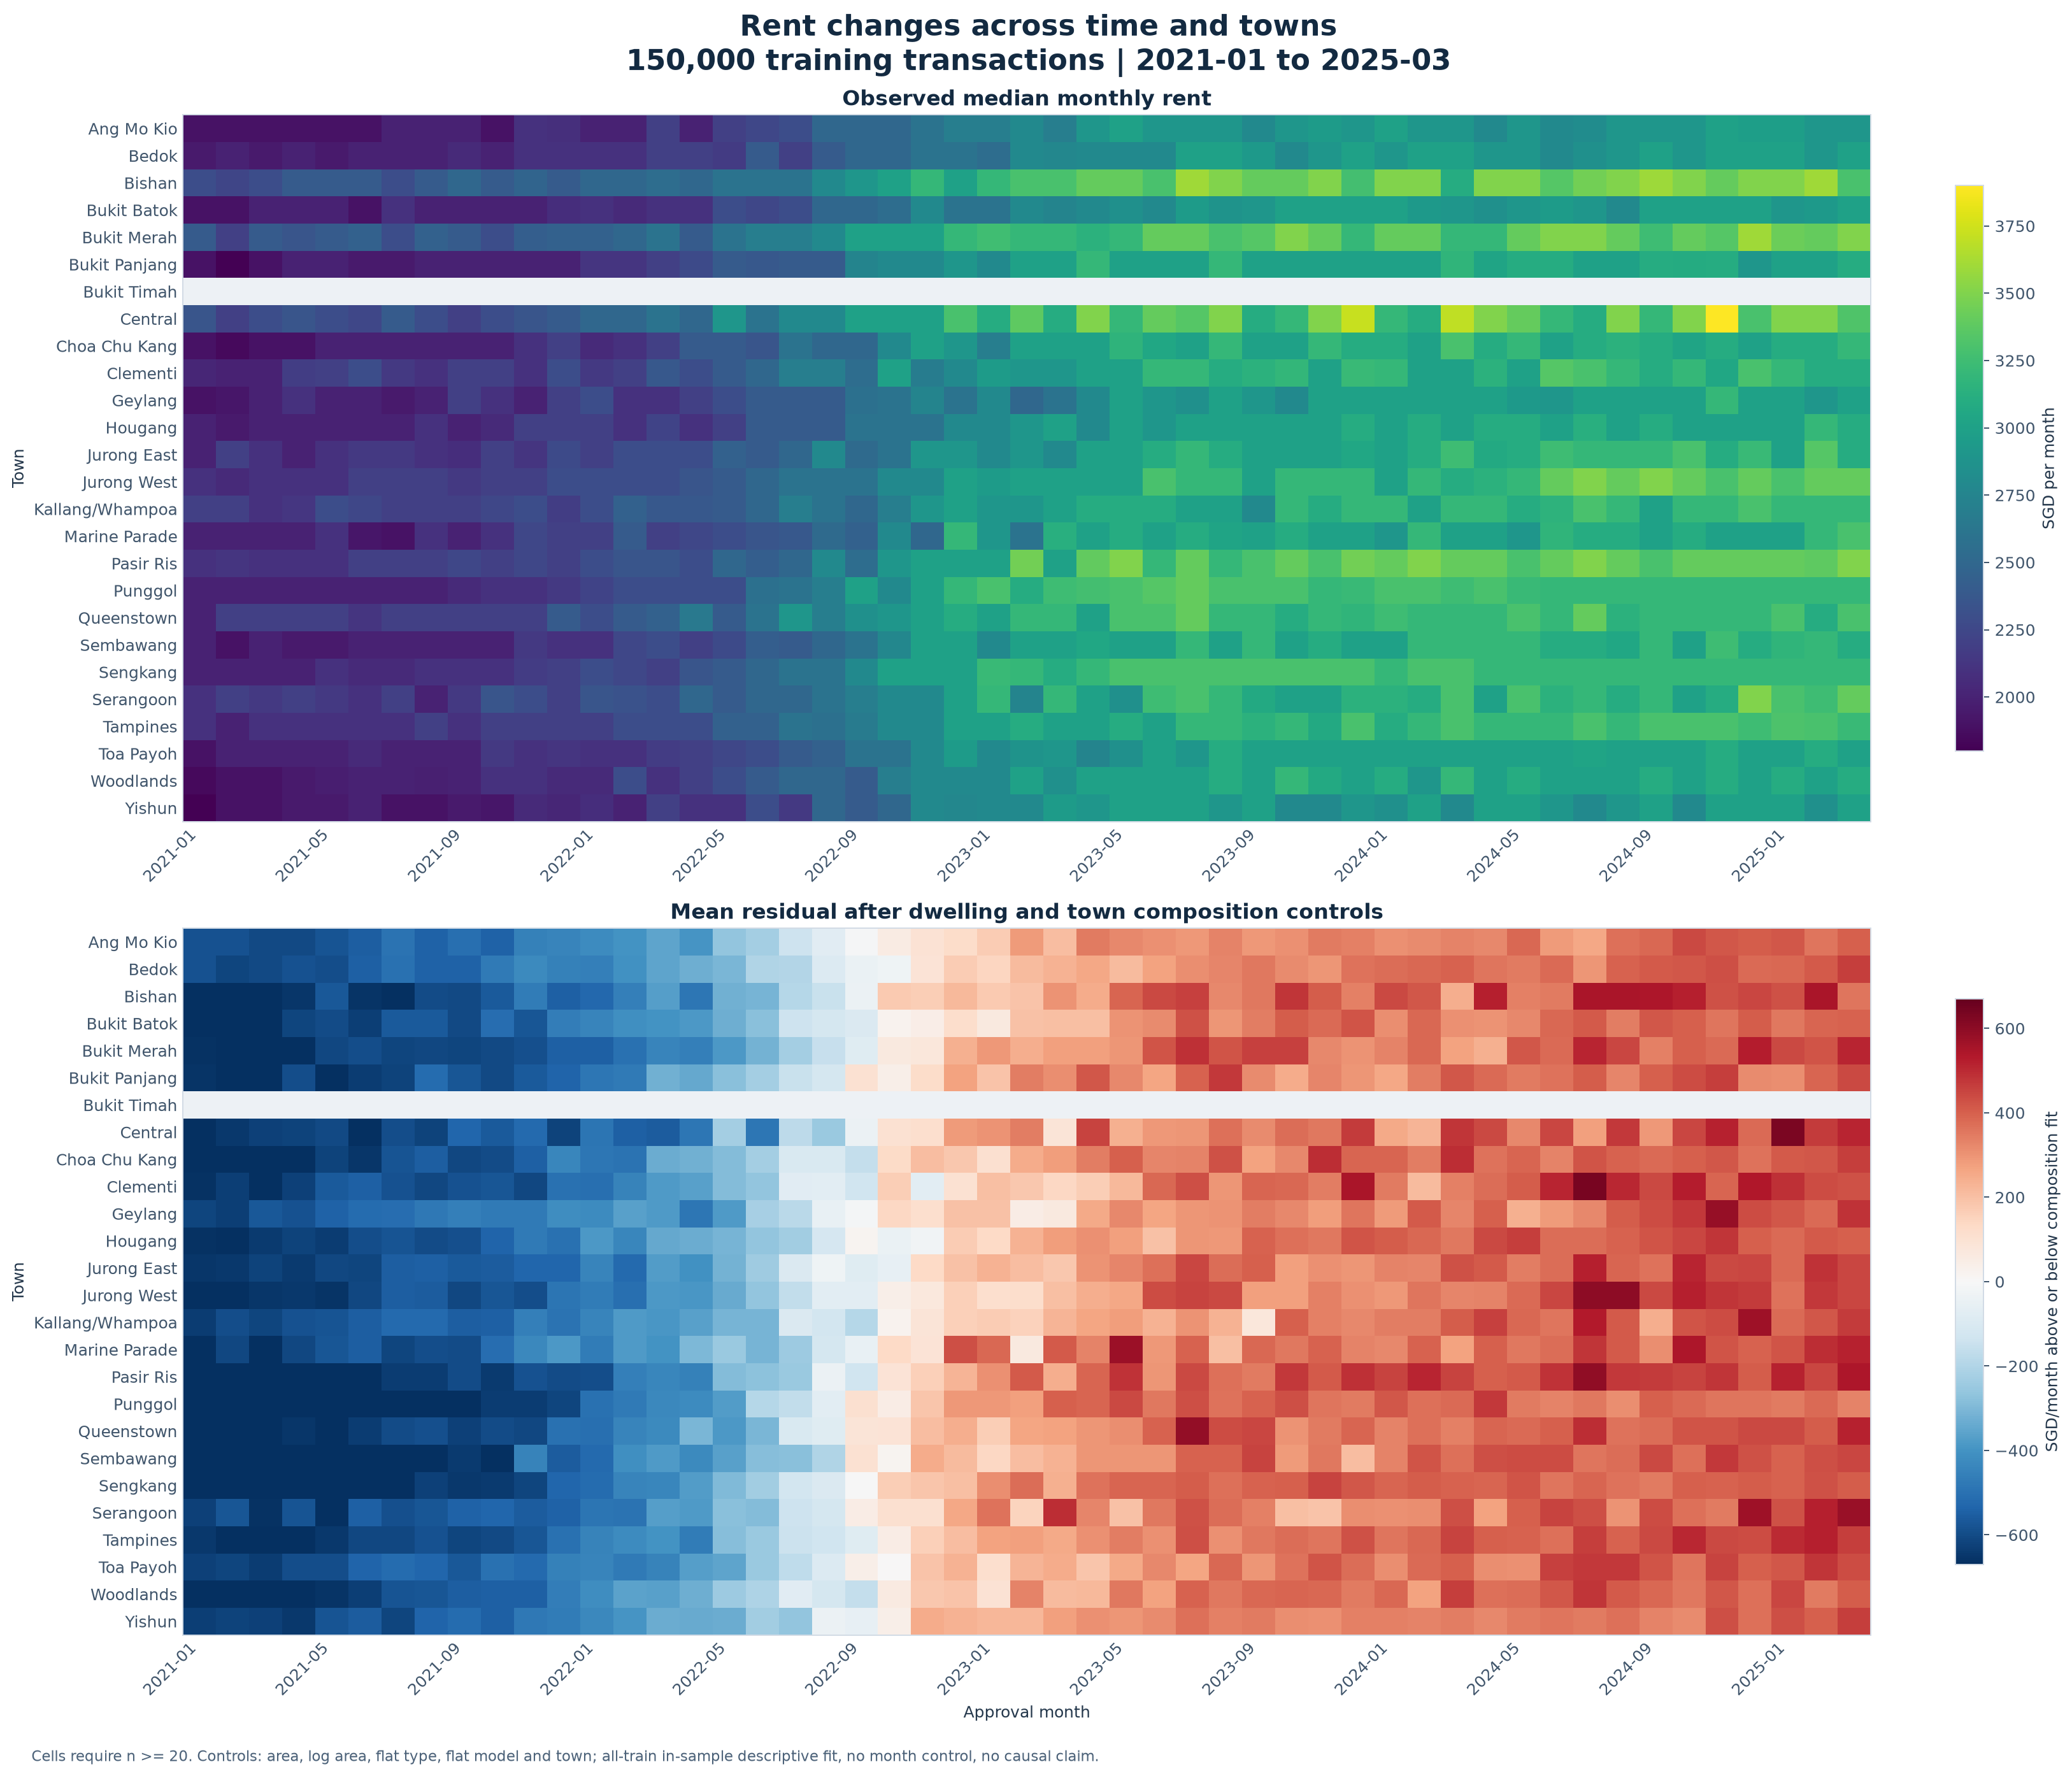
\includegraphics[width=0.96\linewidth,height=0.78\textheight,keepaspectratio]{images/distribution_02_month_town.png}
\\[0.35em]
\refstepcounter{figure}%
{\small Figure~\thefigure: Monthly town distributions: raw rent and composition-adjusted residuals, with sample coverage.}%
\label{fig:rebuiltdistributiontime}%
}

The geographic display has 8,134 blocks with at least five observed rentals. Each block contributes one plotted rent/area summary. The middle panel counts different observed eligible blocks in each spatial cell.

\placefig{%
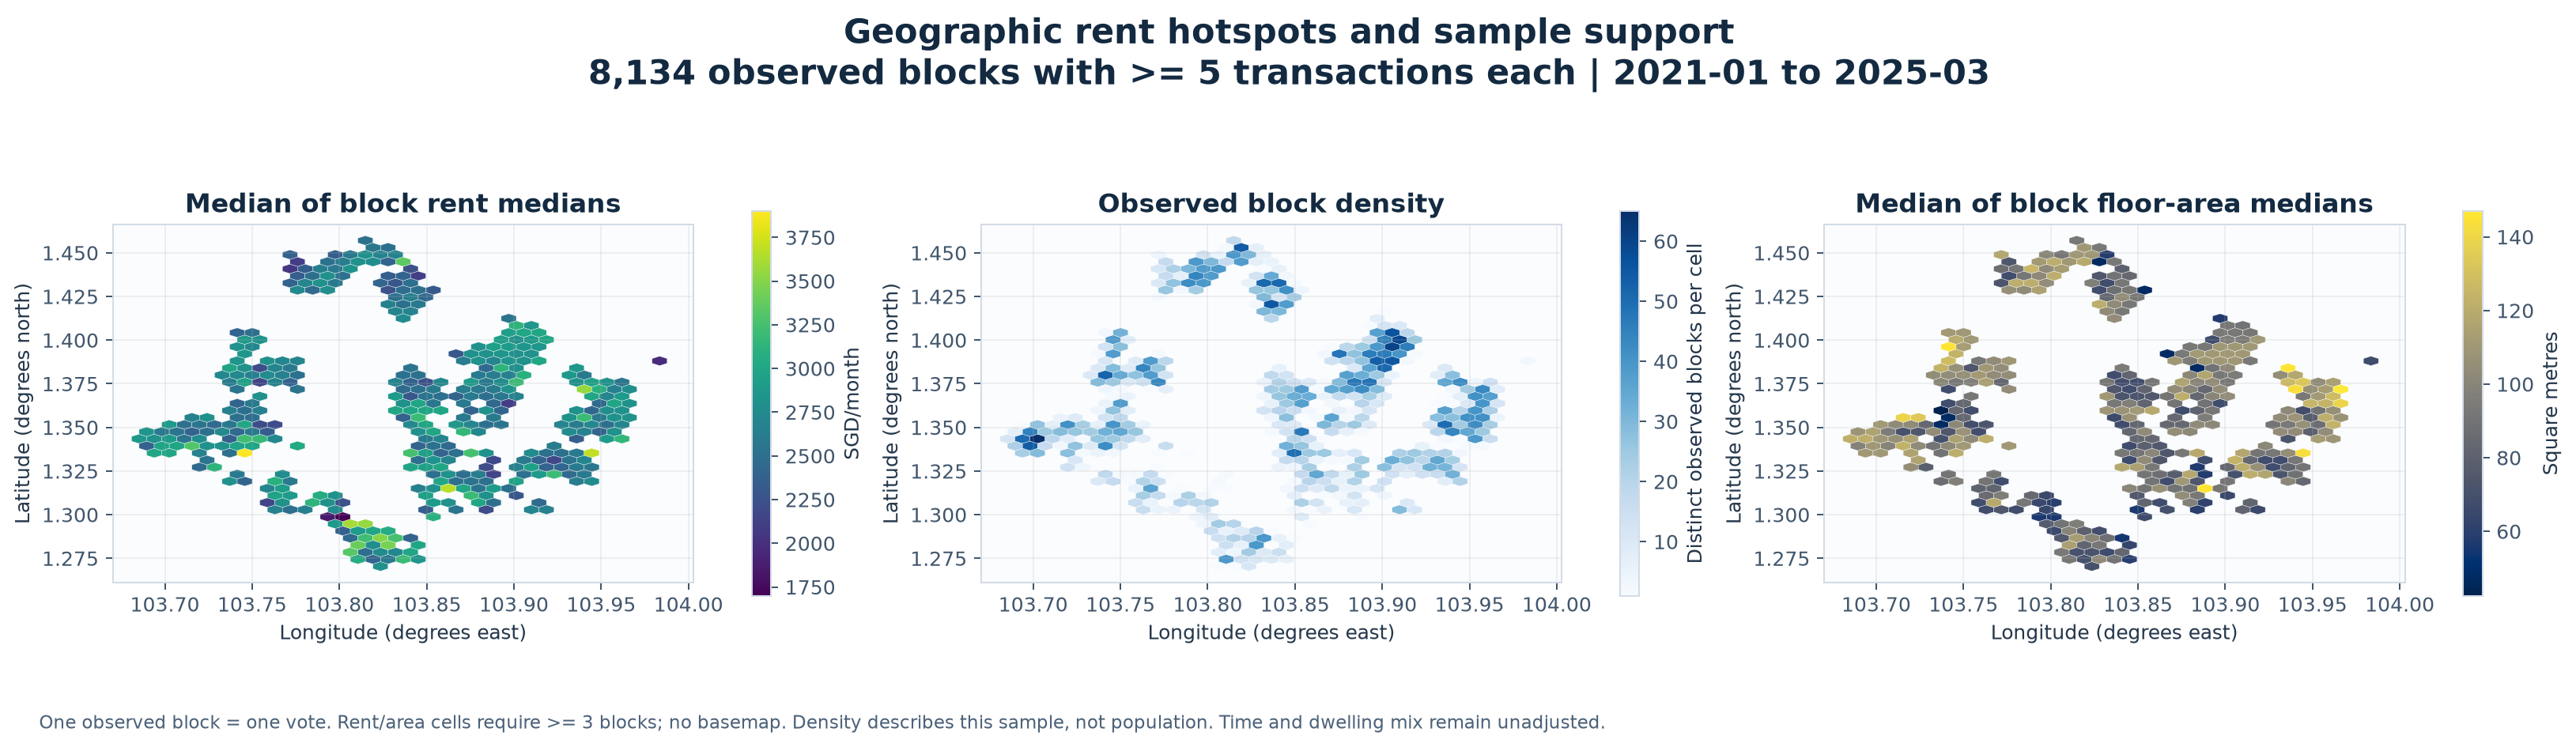
\includegraphics[width=1\linewidth,height=0.78\textheight,keepaspectratio]{images/distribution_03_geo_hotspots.png}
\\[0.35em]
\refstepcounter{figure}%
{\small Figure~\thefigure: Block-level rent, counts of different observed blocks per spatial cell, and area.}%
\label{fig:rebuiltdistributiongeo}%
}

\paragraph{Original dwelling attributes.}
The separate original-dwelling panel compares area and lease-age bands by flat type and shows flat-model median rent beside sample count. Cells with fewer than 50 observations are masked while their counts remain visible. It uses full training data for description, so larger area, different flat types, lease cohorts and flat models must be interpreted together with geography and month rather than as isolated causal premiums. The underlying dwelling-bin and flat-model tables retain all groups.

\subsection{How the auxiliary tables meet the rental features}

The saved tables contain only the new columns, in source-row order, so the original rental fields are concatenated back at training time.
Stations, schools, and malls have coordinates but no block number.
The block table is the hub: it has both an address and coordinates, and every later spatial column starts from that join.

\paragraph{Block attributes and age.}
The rental row is left-joined to the block file on
\begin{equation}
\texttt{block\_key}
=
\mathrm{norm}(\texttt{BLOCK})
\mathbin{\Vert}
\mathrm{norm}(\texttt{STREET}),
\end{equation}
where \texttt{norm} strips, lowercases, and collapses spaces.
The key matches every training and test row, and the row count does not change.
The copied fields are latitude, longitude, postal code (\texttt{NIL} becomes null), maximum floor, year of completion, subzone, planning area, and region.
Building age is the approval year minus the completion year.
Lease age uses \texttt{LEASE\_COMMENCE\_DATE} instead.
A third column is the gap between those two years, and a product of building age with a Central Region flag lets a linear model treat age differently in the centre.
The motivation is that town alone does not say whether the block is central, new, or tall, and the same completion year is a different age in 2021 and in 2026.
Figure~\ref{fig:blocks} shows the joined region and those age and floor distributions.

\placefig{%
\begin{minipage}[t]{0.38\textwidth}
\centering
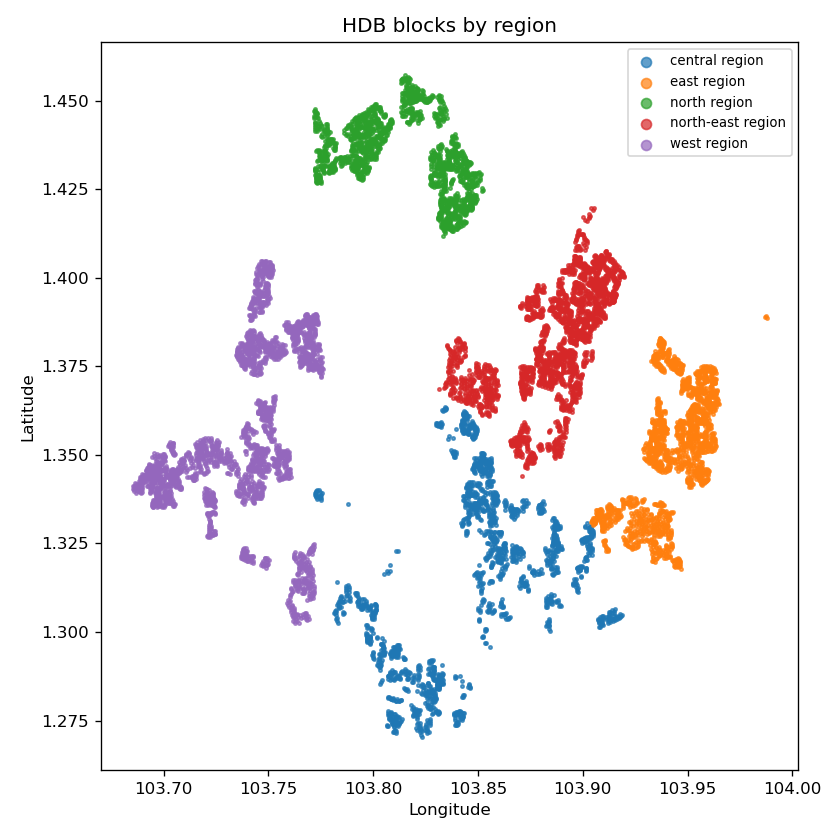
\includegraphics[width=\linewidth]{images/blocks_region_map.png}\\[0.2em]
{\small (a) Region after the address join.}
\end{minipage}\hfill
\begin{minipage}[t]{0.56\textwidth}
\centering
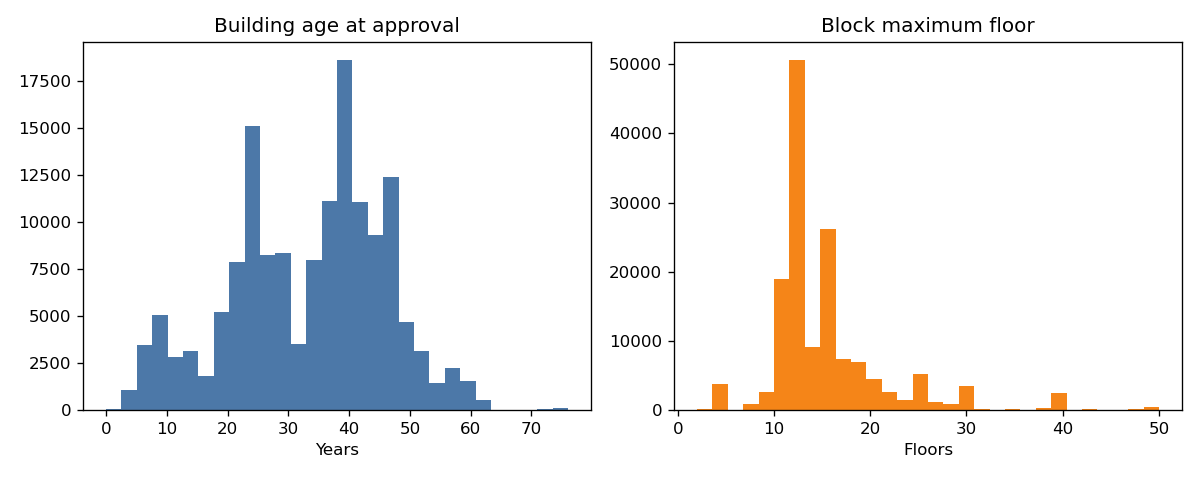
\includegraphics[width=\linewidth]{images/blocks_age_floor.png}\\[0.2em]
{\small (b) Age at approval, and maximum floor.}
\end{minipage}\\[0.35em]
\refstepcounter{figure}%
{\small Figure~\thefigure: Block attributes copied onto the rental rows.}%
\label{fig:blocks}%
}

\paragraph{MRT.}
Distances use Haversine with Earth radius 6{,}371\,km.
The open trunk set is stations with status \texttt{open} whose code prefix is NS, NE, CC, DT, TE, EW, or CG.
The two open Changi Airport (\texttt{CG}) stations are labelled EW.
For each block we store the nearest trunk station's distance, code, normalized name, and line, plus the nearest station and distance on each of the six lines, and the number of trunk codes within 0.5, 1, and 2\,km.
Ties closer than $10^{-6}$\,km keep the lexicographically smallest code.
Planned stations, and prefixes CR, JE, JS, JW, and CP, stay in their own distance columns so they cannot shrink the open-station distance.
A flag is 1 when the nearest trunk station's name has at least two codes.
The motivation is access: a flat near a station is easier to commute from, one distance cannot tell which corridor that station serves, and a count separates a single station from a cluster.
Figure~\ref{fig:mrt} shows that most rentals are within about 1\,km of some trunk station, that 0.5\,km is often empty, and that the North East Line is farther than the East--West Line.

\placefig{%
\begin{minipage}[t]{0.48\textwidth}
\centering
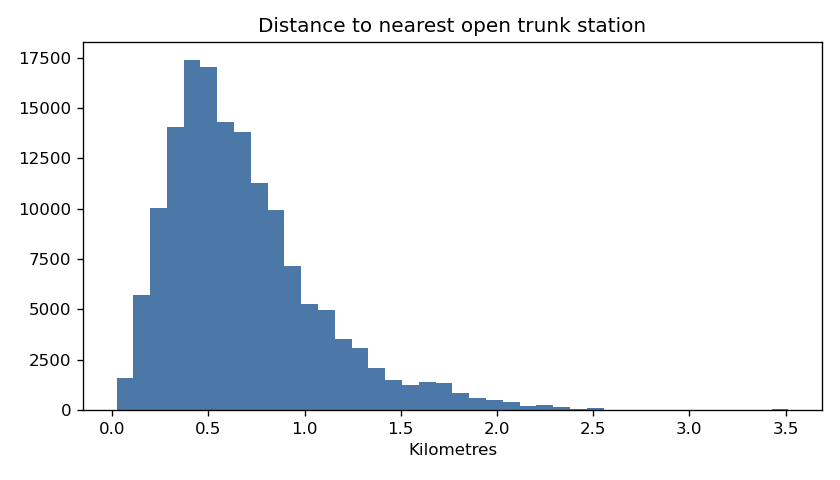
\includegraphics[width=\linewidth]{images/mrt_nearest_trunk.png}\\[0.2em]
{\small (a) Nearest open trunk station.}
\end{minipage}\hfill
\begin{minipage}[t]{0.48\textwidth}
\centering
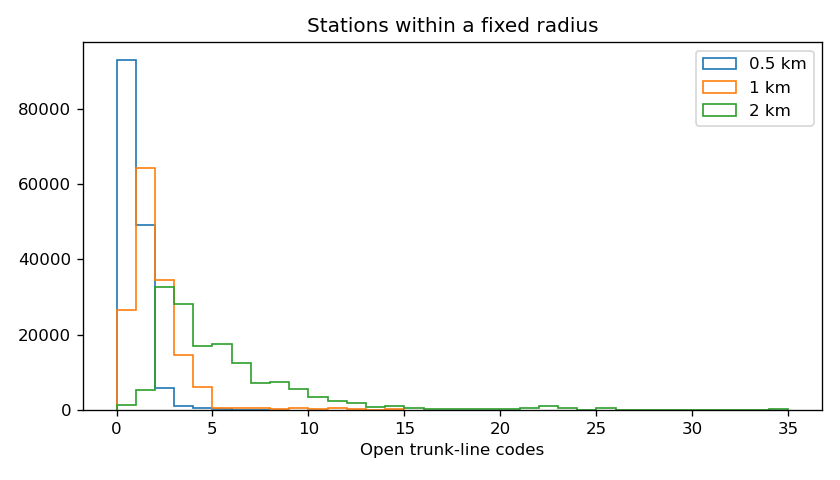
\includegraphics[width=\linewidth]{images/mrt_radius_counts.png}\\[0.2em]
{\small (b) Trunk-line codes within 0.5, 1, and 2\,km.}
\end{minipage}\\[0.45em]
\begin{minipage}[t]{0.58\textwidth}
\centering
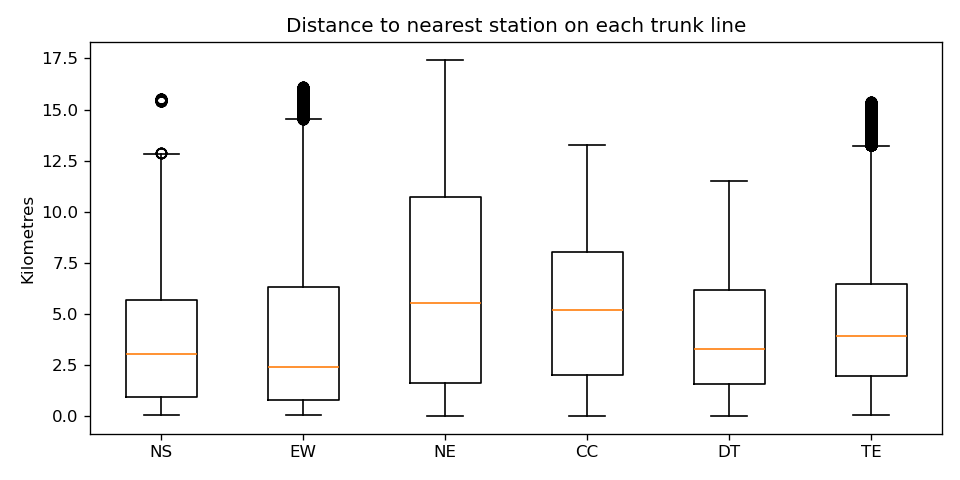
\includegraphics[width=\linewidth]{images/mrt_line_distances.png}\\[0.2em]
{\small (c) Nearest station on each trunk line.}
\end{minipage}\\[0.35em]
\refstepcounter{figure}%
{\small Figure~\thefigure: MRT access. An interchange is counted once per code.}%
\label{fig:mrt}%
}

\paragraph{Schools and malls.}
Primary schools are rows with \texttt{MAINLEVEL\_CODE} equal to \texttt{primary} (179 schools).
Secondary schools are the two strings \texttt{secondary (s1-s5)} and \texttt{secondary (s1-s4)} (133 schools).
Each set contributes a nearest distance, the normalized school name, and a count within 1\,km; primary schools also have a 2\,km count.
All 337 schools add one more nearest distance, name, and 1\,km count.
All 113 malls contribute the nearest distance, normalized name, and counts within 1 and 2\,km.
Names are kept because those tables have no code, and the normalized name is unique.
The motivation is daily convenience: households pay for a short walk to a primary school or a shop, and a count distinguishes one neighbour from several.
Figure~\ref{fig:amenity} shows schools packed closer than malls, and many rentals with no mall inside 1\,km.

\placefig{%
\begin{minipage}[t]{0.60\textwidth}
\centering
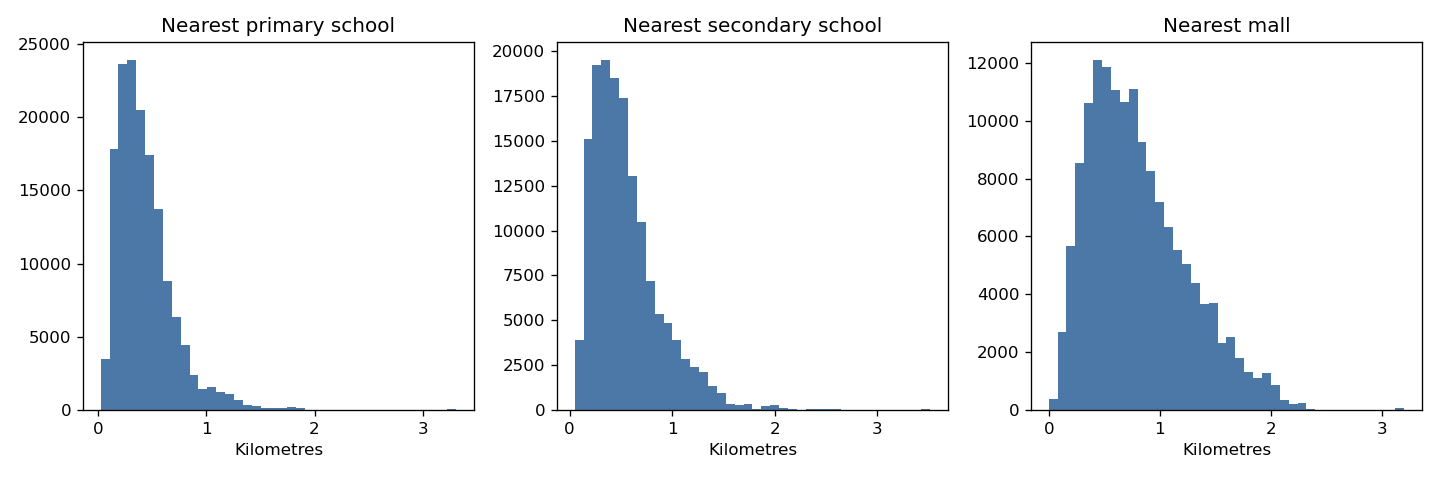
\includegraphics[width=\linewidth]{images/amenity_distances.png}\\[0.2em]
{\small (a) Nearest primary school, secondary school, and mall.}
\end{minipage}\hfill
\begin{minipage}[t]{0.36\textwidth}
\centering
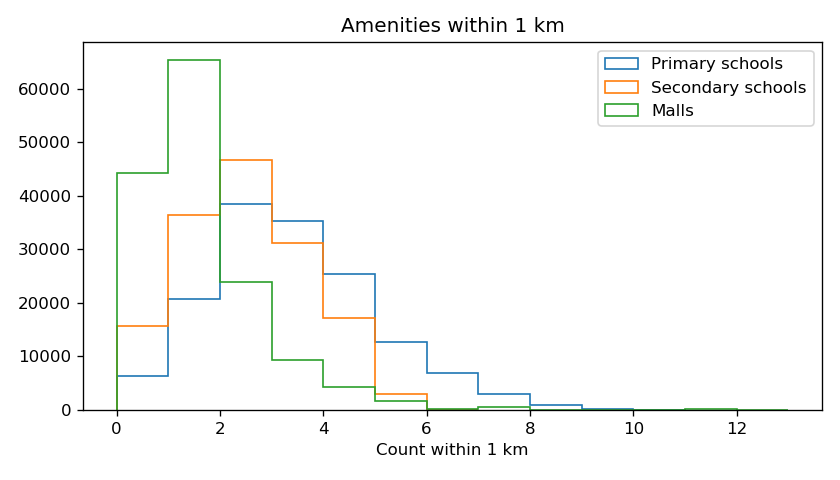
\includegraphics[width=\linewidth]{images/amenity_counts_1km.png}\\[0.2em]
{\small (b) Counts within 1\,km. Zero is a real zero.}
\end{minipage}\\[0.35em]
\refstepcounter{figure}%
{\small Figure~\thefigure: Schools and malls around the training rentals.}%
\label{fig:amenity}%
}

\paragraph{Density and a fixed downtown point.}
The number of other HDB blocks within 500\,m uses the same block coordinates, excluding the block itself.
The town centroid is the mean latitude and longitude of blocks in that town, and each block is measured to its own centroid.
Distance to the CBD is Haversine to the fixed Raffles Place coordinate $(1.283889, 103.851389)$, taken from station codes \texttt{ns26} and \texttt{ew14}.
A log of the nearest trunk distance, $\ln(d+0.001)$, gives nearby changes more weight than a linear model would give the raw kilometres.
The motivation is position inside a town and on the island: two flats in the same town can still sit at the edge or next to downtown.

\paragraph{COE and stocks.}
COE amounts are parsed by stripping dollar signs and commas.
Each category-month uses bidding round 2, or round 1 if round 2 is absent.
A rental in month $T$ receives the premium, the change from $T-2$ to $T-1$, and bids divided by quota, all from month $T-1$.
Categories A, B, and E have those three columns; category A also has the mean of $T-1$, $T-2$, and $T-3$; category C has only the lagged premium.
Stock features use month-end adjusted closes.
The bank basket is the equal-weight mean of \texttt{D05.SI}, \texttt{O39.SI}, and \texttt{U11.SI}; the property basket is \texttt{C09.SI}, \texttt{U14.SI}, and \texttt{9CI.SI}.
A month is used only when all three symbols have a close, and the rental again sees month $T-1$, both as a level and as that month's return.
The motivation is a market-wide shift that floor area and town cannot express: dearer car quotas or weaker bank shares may coincide with tighter household budgets.
Figure~\ref{fig:market} shows that both series are constant across flats approved in the same month.

\placefig{%
\begin{minipage}[t]{0.48\textwidth}
\centering
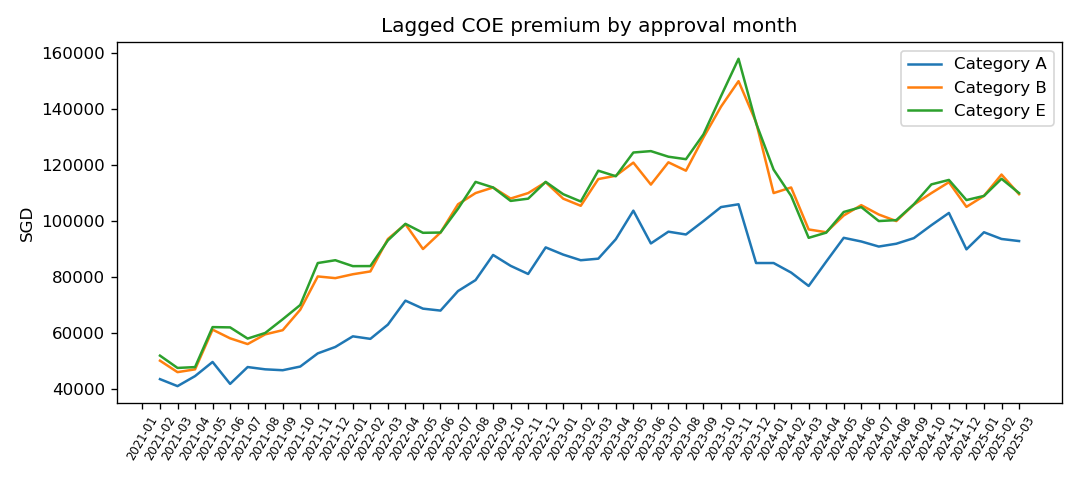
\includegraphics[width=\linewidth]{images/coe_monthly.png}\\[0.2em]
{\small (a) Lagged COE premium.}
\end{minipage}\hfill
\begin{minipage}[t]{0.48\textwidth}
\centering
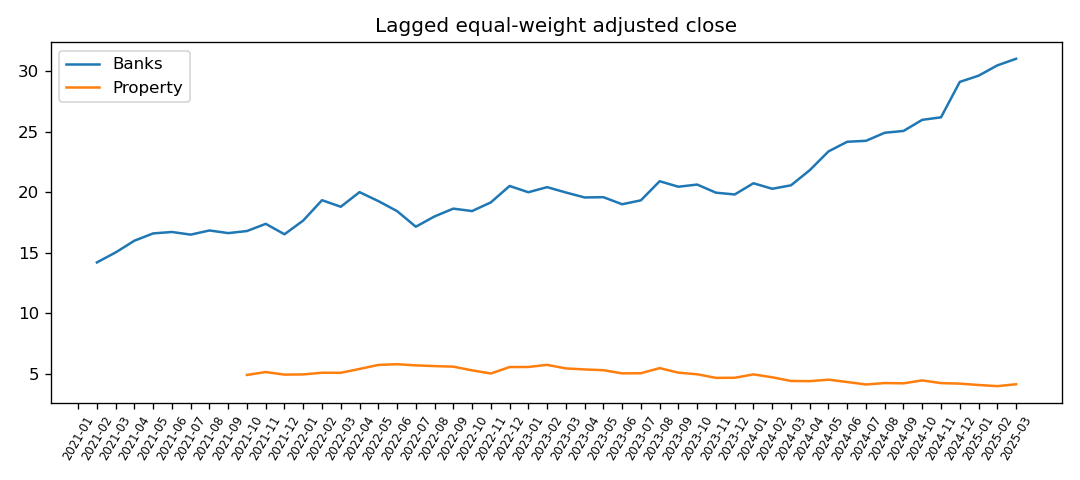
\includegraphics[width=\linewidth]{images/stock_baskets_monthly.png}\\[0.2em]
{\small (b) Lagged bank and property baskets.}
\end{minipage}\\[0.35em]
\refstepcounter{figure}%
{\small Figure~\thefigure: Month-level series shared by every flat approved in that month.}%
\label{fig:market}%
}

\paragraph{Group-mean rents.}
Six columns are target encodings.
For a row in month \(T\), only training rents from \(T-1\), \(T-2\), and \(T-3\) are used:
\begin{equation}
\frac{n\,\bar r_g + 20\,\bar r}{n + 20}.
\end{equation}
Here \(\bar r_g\) is the group mean inside that window, \(n\) is the number of those rows, and \(\bar r\) is the island-wide mean inside the same three months.
If \(n=0\), the value is \(\bar r\).
January 2021 has none of those months in the file, so all six columns are null.
February 2021 uses January only.
The groups are the first two digits of the postal code, the legacy district D01--D28 implied by those digits, \texttt{nearest\_mall\_name}, \texttt{nearest\_open\_mrt\_code}, \texttt{nearest\_primary\_name}, and \texttt{nearest\_secondary\_name}.
The sector and district strings are not stored.
The motivation is the recent local rent level: a mean accumulated since 2021 would still carry old rent levels into 2025, while the previous quarter moves with the market. Shrinkage keeps a thin quarter from being dominated by a few leases.
The month-by-group heatmaps in \texttt{outputs/figures/heatmap\_*.png} draw this formula even when that month has no rental in the group.
A cell is blank only when the three-month window contains no training rents.
The maps in \texttt{outputs/figures/maps/} place the same values on an OpenStreetMap background for each June and December whose window overlaps the training months.
Each land cell takes the colour of its single nearest mall, primary school, or open MRT station, and each map has its own colour scale.
Figure~\ref{fig:mrt-map} is the June 2025 MRT map.
Its window is March, April, and May 2025, and the training file ends in March 2025, so the colours use March 2025 rents only.
A darker patch is the service area of one station whose recent rents were higher. The scale belongs to this file alone.

\placefig{%
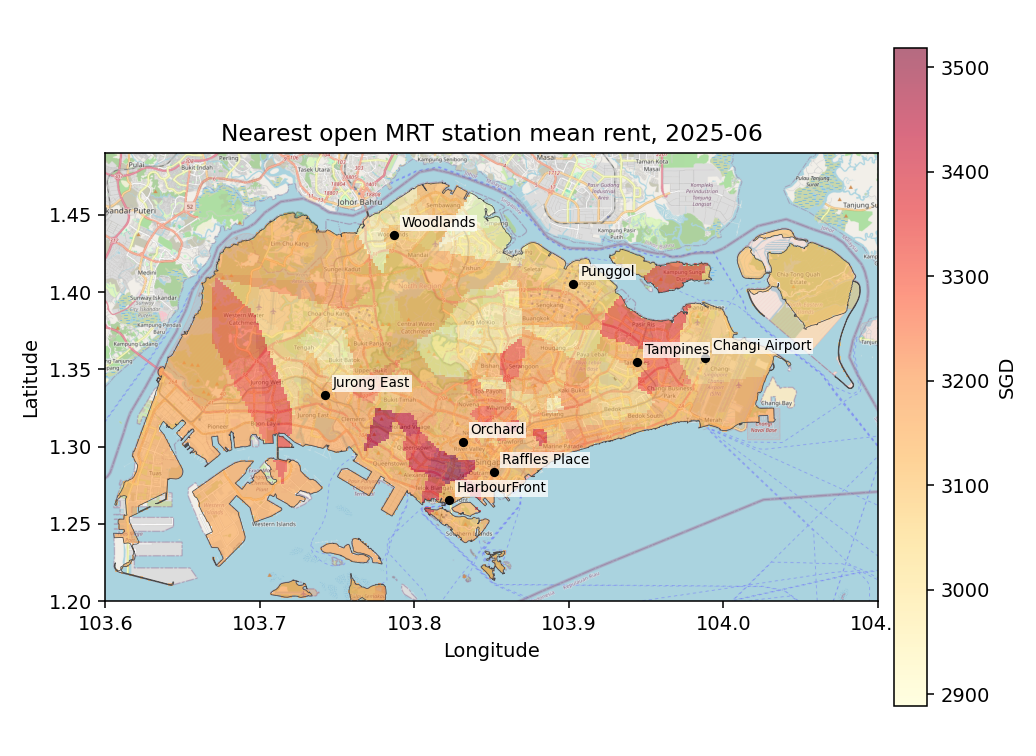
\includegraphics[width=0.92\linewidth]{./outputs/figures/maps/map_mrt_2025-06.png}\\[0.35em]
\refstepcounter{figure}%
{\small Figure~\thefigure: Nearest open MRT station, June 2025. Colour is the smoothed mean of training rents in the previous three months for that station. Each area is one station.}%
\label{fig:mrt-map}%
}

\subsection{Limits of the built columns}

\begin{itemize}
\item \texttt{MAX\_FLOOR} is the top floor of the block. Values of $-1$ on floor and completion year are sentinels and are stored as null (159 training rows, no test rows).
\item The MRT file has no opening date. A station marked open may have opened after January 2021. Planned stations and future-line prefixes are kept out of the open-station distance.
\item About 20 MRT longitudes have only one to three decimal places. Switching from Haversine to SVY21 does not repair that.
\item Great-circle distance is not walking time. School and mall tables have no opening dates, and the school table has no university.
\item COE and stock columns are constant within an approval month. January 2021 COE lags are null because December 2020 is missing. The property basket is missing on early training rows because one constituent starts later.
\item Group means are target encodings of the previous three months of rents, not properties of a mall, station, or school. January 2021 is null. A mall mean covers rentals for which that mall is the nearest mall, not every flat inside a radius.
\item Empty postal codes (285 blocks) have no postal-sector group and fall back to that quarter's island-wide mean once the three-month window contains any training rent.
\end{itemize}

\subsection{How the features will be tested}

This check has not been run.
Train on earlier approval months and validate on later months, and use that same split for every model.
Do not fit group means, or any other rent statistic, on the validation months.

Start with the mean training rent, then a linear model on the original rental fields only.
Add one auxiliary family at a time: block and age, MRT, schools and malls, density and CBD distance, COE and stocks, then group-mean rents.
Repeat the same feature sets with XGBoost and a multilayer perceptron.
Trees can split raw distances and categories; the linear model and the MLP depend more on scaling and on the explicit transforms.
Use family ablation for groups of columns, and linear coefficients or permutation importance for single columns.
A column is kept only if it lowers validation RMSE under this split.
An in-sample correlation with rent is not enough, especially for the group means, which repeat recent rents unless the time split is enforced.

\subsection{Locked temporal comparisons and information timing}
Development trains through April 2022, October 2022 and April 2023; the corresponding validation windows are May--October 2022, November 2022--April 2023 and May--October 2023. The long assessment trains through October 2023 and evaluates November 2023--March 2025. 
The original-address baseline includes normalized block and street as well as dwelling, town and calendar features. Mean and Ridge checks accompany the matched CatBoost comparisons. All tree configurations share the recorded hyperparameters. A positive addition gain is original-address RMSE minus augmented RMSE; a positive removal cost is ablated RMSE minus full-model RMSE. Development RMSE pools total squared error and row count across the three folds, rather than averaging three RMSEs.

The cutoff-frozen scenario holds validation macro descriptors at the start-month feature vector, which contains only observations available by the preceding cutoff. The provided-lagged scenario conditions each rental month on supplied observations from the preceding completed month. It is a batch prediction setting, not a years-ahead forecast without future covariates. Missing source observations are not invented. Stock PCA is learned with one row per training month, not with repeated rental rows.

\paragraph{Cutoff-frozen macro.}
\begin{center}
\small
\begin{tabular}{lrr}
\toprule
Configuration & Dev. pooled RMSE & 17m RMSE \\
\midrule
Training mean & 939.64 & 894.19 \\
Ridge original + address & 632.91 & 677.64 \\
Ridge all auxiliary & 615.95 & 544.21 \\
Original dwelling & 640.49 & 509.53 \\
Original + address & 627.84 & 501.83 \\
All main auxiliary & 631.09 & 517.51 \\
add mrt & 622.58 & 499.53 \\
Adjusted-price sensitivity & 640.58 & 520.05 \\
\bottomrule
\end{tabular}
\end{center}

\paragraph{Provided lagged macro.}
\begin{center}
\small
\begin{tabular}{lrr}
\toprule
Configuration & Dev. pooled RMSE & 17m RMSE \\
\midrule
Training mean & 939.64 & 894.19 \\
Ridge original + address & 632.91 & 677.64 \\
Ridge all auxiliary & 613.40 & 509.29 \\
Original dwelling & 640.49 & 509.53 \\
Original + address & 627.84 & 501.83 \\
All main auxiliary & 643.79 & 553.50 \\
add mrt & 622.58 & 499.53 \\
Adjusted-price sensitivity & 661.29 & 549.25 \\
\bottomrule
\end{tabular}
\end{center}

Among the predefined main CatBoost configurations (excluding retrospective adjusted-price sensitivity), the lowest pooled development RMSE belongs to add\_mrt. This ranking uses development results only.

\placefig{%
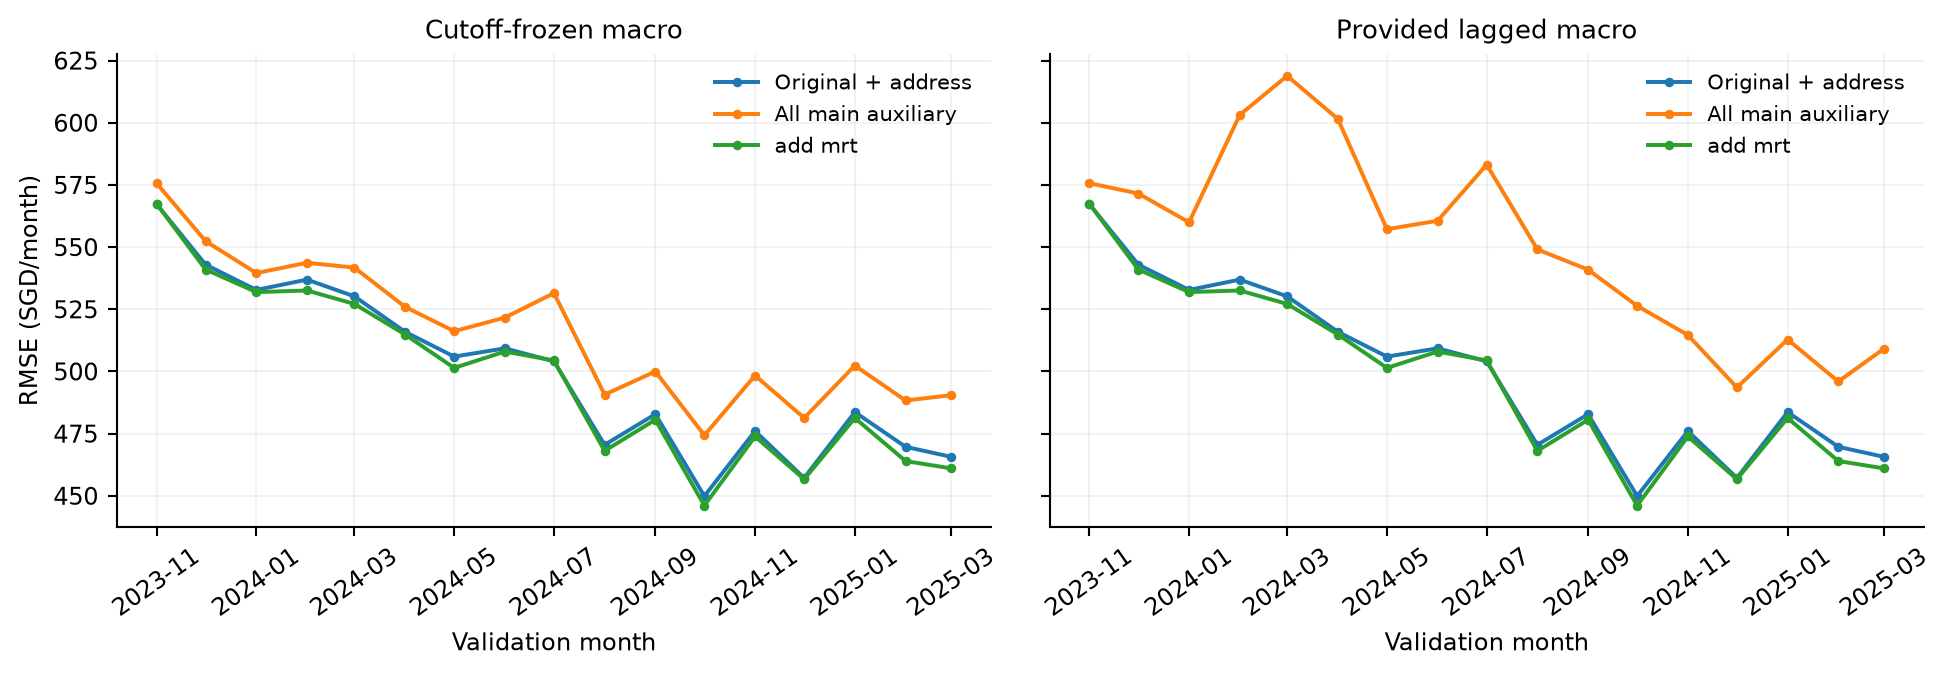
\includegraphics[width=0.96\linewidth,height=0.78\textheight,keepaspectratio]{images/rebuilt_17month_errors.png}
\\[0.35em]
\refstepcounter{figure}%
{\small Figure~\thefigure: Monthly error across the locked 17-month assessment.}%
\label{fig:rebuiltmonthly}%
}

\subsection{Conditional associations and complete stock coverage}
Each numeric spatial exposure is tested separately after controls for area, log area, lease age, flat type, flat model, town and approval-month fixed effects, using development data through October 2023. The spatial exposures are not jointly included in this screen. Intervals cluster by address. These describe conditional association, not causal facility premiums: unobserved unit floor, renovation, household composition and neighbourhood differences can remain. Coefficients below are SGD per original feature unit. The distance curves show zero-centered adjusted rent residuals in quantile bins, without adding back baseline rent or choosing a reference band. Their pointwise address-cluster intervals omit control-fit uncertainty.

\begin{center}
\small
\begin{tabular}{lrr}
\toprule
Spatial variable (unit) & SGD/unit & 95\% interval (SGD) \\
\midrule
Maximum block floor (floor) & +6.49 & [5.25, 7.73] \\
Building age (year) & -1.36 & [-4.86, 2.13] \\
CBD distance (km) & -31.22 & [-37.04, -25.40] \\
Open MRT distance (km) & -132.52 & [-147.89, -117.16] \\
Mall distance (km) & -97.26 & [-109.04, -85.49] \\
Primary distance (km) & -22.50 & [-42.27, -2.74] \\
Secondary S1--S4 (km) & -36.82 & [-43.30, -30.35] \\
Secondary S1--S5 (km) & +19.22 & [4.72, 33.71] \\
\bottomrule
\end{tabular}
\end{center}

\placefig{%
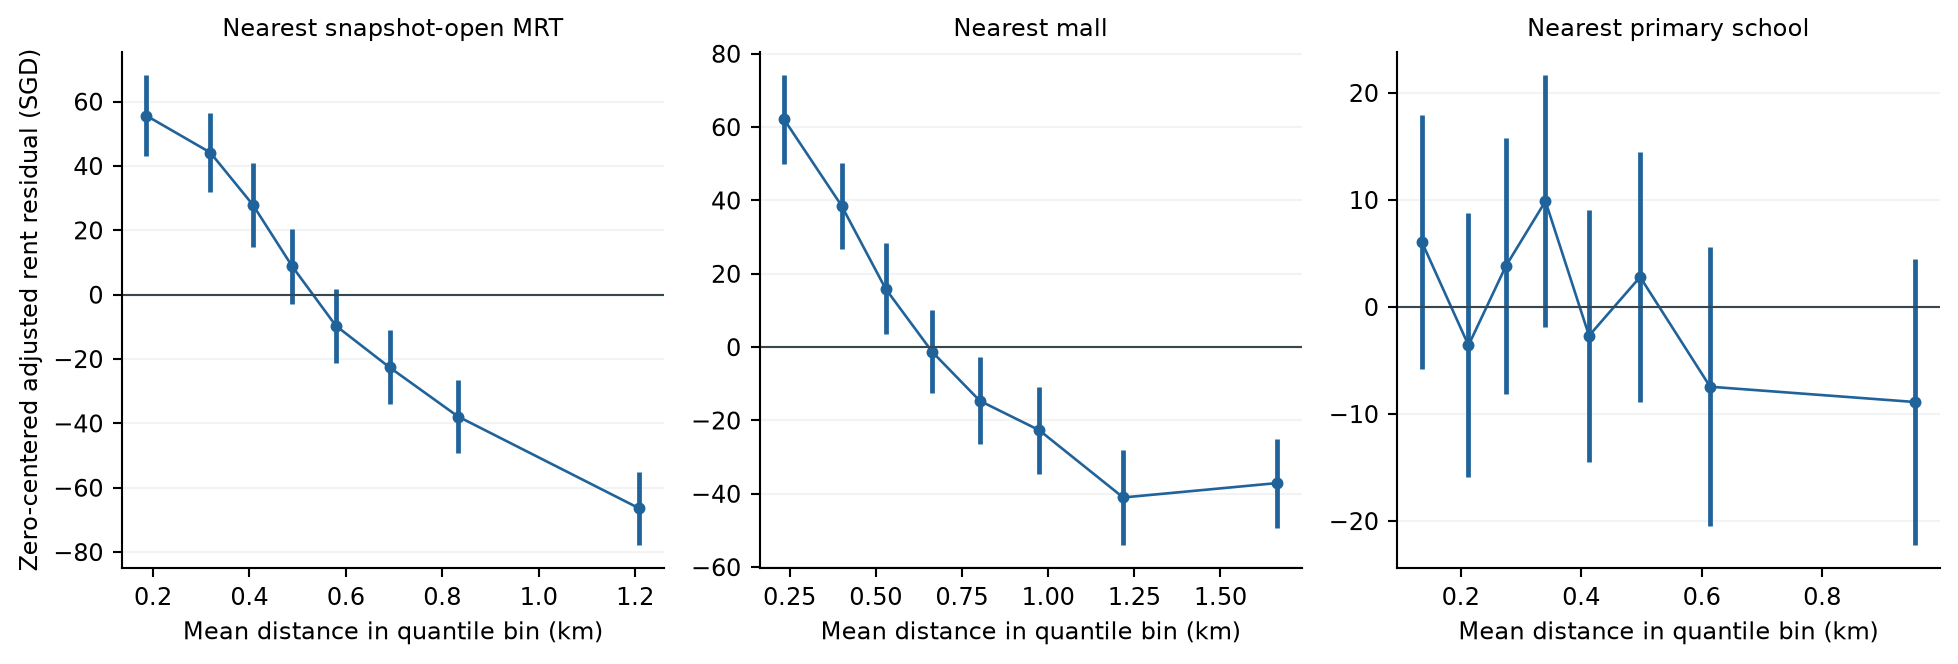
\includegraphics[width=0.96\linewidth,height=0.78\textheight,keepaspectratio]{images/rebuilt_conditional_distance_bands.png}
\\[0.35em]
\refstepcounter{figure}%
{\small Figure~\thefigure: Selected zero-centered adjusted-rent residual curves by distance.}%
\label{fig:rebuiltdistance}%
}

\paragraph{Original and constructed predictors in the fitted model.}
SHAP magnitudes describe attribution in the fitted full model on the recorded assessment sample. They help locate predictive signals such as dwelling attributes, calendar and location.

\placefig{%
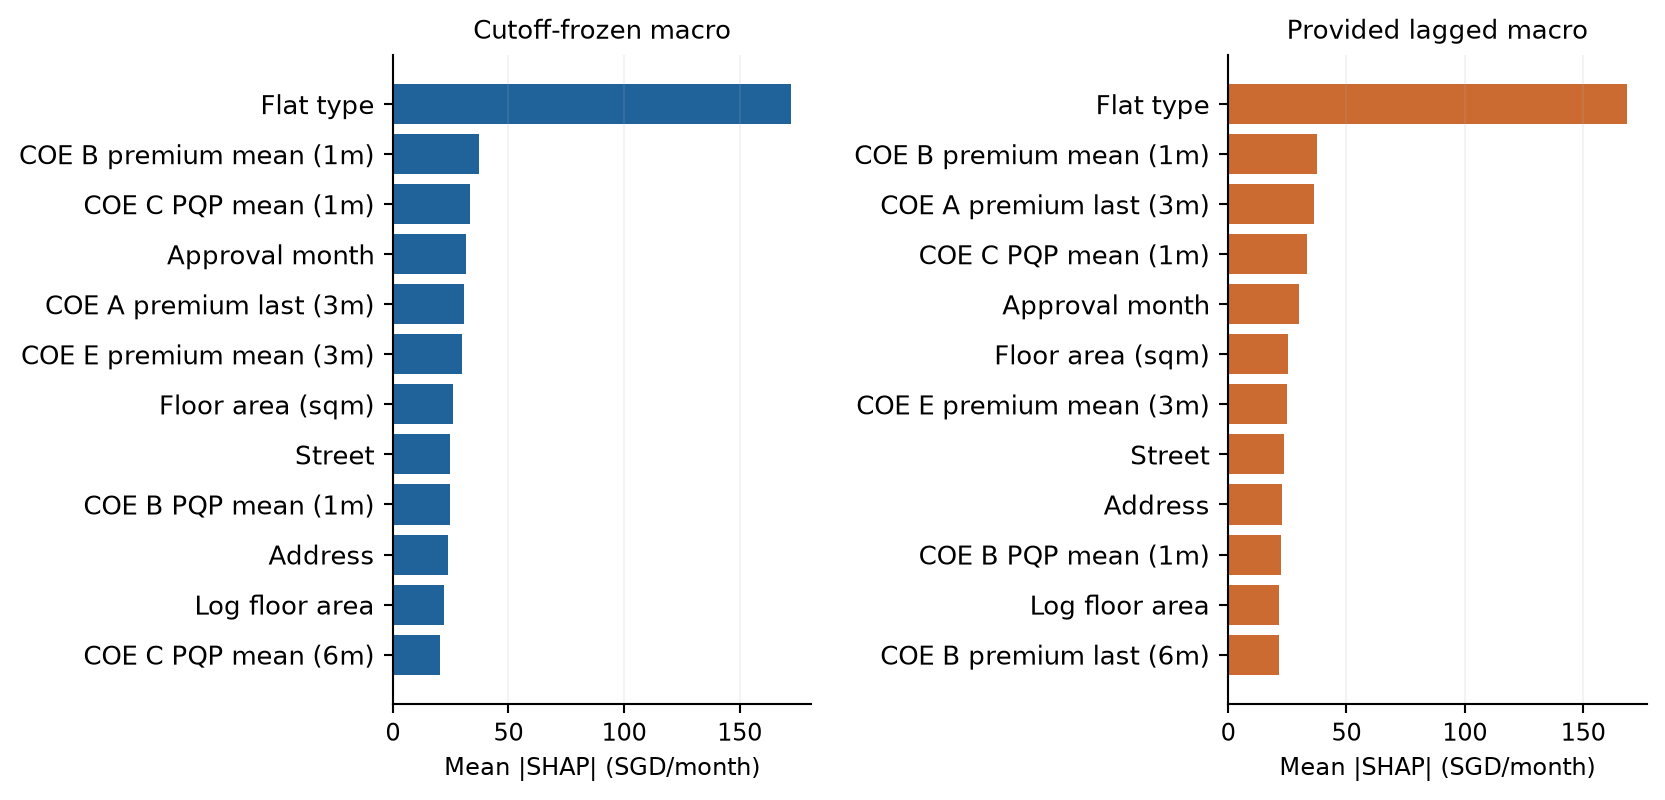
\includegraphics[width=0.96\linewidth,height=0.78\textheight,keepaspectratio]{images/rebuilt_model_attributions.png}
\\[0.35em]
\refstepcounter{figure}%
{\small Figure~\thefigure: Leading full-model attributions on the fixed assessment sample.}%
\label{fig:rebuiltshap}%
}

\section{Core rental data: audit and preprocessing}
\label{sec:preprocessing}

The prediction target is \texttt{MONTHLY\_RENT}.
The core data contain 150{,}000 training records and 50{,}000 test records.
The training file has 10 input fields plus the target, while the test file has the same 10 inputs without the target.
Before feature construction or model fitting, both files are audited for dimensions, data types, missing values, categorical consistency, numerical ranges, duplicate records, and approval-month coverage.
No row is removed during this stage unless there is clear evidence that it is invalid.

\subsection{Initial data audit}

The raw core data contain no missing cells in either train or test.
The main data-quality issues are therefore inconsistent representations, constant columns, unusual records, and the difference in time coverage between the two datasets.

\begin{table}[h]
\centering
\small
\begin{tabular}{lrr}
\toprule
 & Training & Test \\
\midrule
Rows & 150{,}000 & 50{,}000 \\
Input fields & 10 & 10 \\
Missing cells & 0 & 0 \\
Approval period & Jan 2021--Mar 2025 & Mar 2025--Jul 2026 \\
Unique approval months & 51 & 17 \\
\bottomrule
\end{tabular}
\caption{Basic properties of the supplied core rental data.}
\label{tab:core-overview}
\end{table}

The approval-date field also uses different raw formats.
Training dates appear as strings such as \texttt{March-25}, whereas the test file uses strings such as \texttt{2025-03}.
The two formats are therefore parsed explicitly instead of assuming that the same string pattern is used in both files.

The original training and test tables are preserved separately before any modification.
All later deterministic cleaning operations are applied through the same functions so that a category is represented identically in train and test.

\subsection{Categorical normalization}

The categorical fields \texttt{TOWN}, \texttt{BLOCK}, \texttt{STREET}, \texttt{FLAT\_TYPE}, \texttt{FLAT\_MODEL}, and \texttt{FURNISHED} are stripped of leading and trailing spaces, converted to lower case, and reduced to a single internal space.

The largest inconsistency appears in \texttt{STREET}.
The training data contain 1{,}146 raw street labels, but only 576 unique values after case and whitespace normalization.
The test data similarly reduce from 1{,}129 raw labels to 573 normalized street names.
The transformation changes the representation of 30{,}781 training rows and 10{,}482 test rows without changing their semantic location.

\texttt{FLAT\_TYPE} has a second inconsistency.
For example, \texttt{4 room} and \texttt{4-room} describe the same type of flat.
All one- to five-room labels are standardized to the hyphenated form using a deterministic regular-expression rule.
This reduces the training categories from 11 to 6 and modifies 35{,}331 training rows.
The test set already follows the standardized naming convention.

\begin{table}[h]
\centering
\small
\begin{tabular}{lrrrr}
\toprule
Feature & Train before & Train after & Train rows changed & Test rows changed \\
\midrule
\texttt{STREET} & 1{,}146 & 576 & 30{,}781 & 10{,}482 \\
\texttt{FLAT\_TYPE} & 11 & 6 & 35{,}331 & 0 \\
\bottomrule
\end{tabular}
\caption{Main categorical standardization results.}
\label{tab:category-cleaning}
\end{table}

The two fields \texttt{FURNISHED} and \texttt{FEE} are checked in both datasets before removal.
\texttt{FURNISHED} is \texttt{yes} for every record, while \texttt{FEE} is 0 for every record.
Since neither field has any variation across train or test, both are removed from the modeling table.

\subsection{Time and property features}

The approval-date field is converted into a common monthly representation.
Three variables are derived:
\texttt{APPROVAL\_YEAR},
\texttt{APPROVAL\_MONTH},
and a continuous \texttt{MONTH\_INDEX}.
January 2021 is assigned month index 0:
\begin{equation}
\texttt{MONTH\_INDEX}
=
12(\texttt{APPROVAL\_YEAR}-2021)
+
(\texttt{APPROVAL\_MONTH}-1).
\end{equation}

The training values run from 0 to 50, while the test set continues to 66.
This feature preserves the chronological order of rental observations and allows the later model to represent the broad market trend.
The separate year and month fields are also retained because they can capture effects that are not represented by one continuous variable alone.

A building identifier is constructed as
\begin{equation}
\texttt{BUILDING}
=
\texttt{BLOCK}
\mathbin{\Vert}
\texttt{STREET}.
\end{equation}
Block number alone is ambiguous because the same number can occur on different streets.
The combined identifier gives a more specific property-location category.
There are 9{,}406 unique buildings in the training data and 8{,}940 in the test data.

Lease age is calculated relative to the rental approval year rather than to the current year:
\begin{equation}
\texttt{LEASE\_AGE}
=
\texttt{APPROVAL\_YEAR}
-
\texttt{LEASE\_COMMENCE\_DATE}.
\end{equation}
This makes the feature consistent for observations from different years.

One training row has a lease commencement year later than its rental approval year.
Instead of deleting the entire observation, an indicator
\texttt{LEASE\_AGE\_INVALID} is set to 1 and only its derived lease age is stored as null.
No such case occurs in the test set.

\begin{table}[h]
\centering
\small
\begin{tabular}{lll}
\toprule
Derived feature & Source & Motivation \\
\midrule
\texttt{APPROVAL\_YEAR} & approval date & long-term time trend \\
\texttt{APPROVAL\_MONTH} & approval date & calendar month effect \\
\texttt{MONTH\_INDEX} & year and month & continuous temporal order \\
\texttt{BUILDING} & block and street & specific location identifier \\
\texttt{LEASE\_AGE} & approval year and lease year & age proxy at rental time \\
\texttt{LEASE\_AGE\_INVALID} & lease-age check & preserve logical anomaly information \\
\bottomrule
\end{tabular}
\caption{Features derived during core preprocessing.}
\label{tab:derived-core-features}
\end{table}

After these variables are constructed, the original string-valued \texttt{RENT\_APPROVAL\_DATE} is removed because the same information is represented consistently by the derived time features.

\subsection{Duplicates and numerical anomalies}

Duplicate records are inspected but are not automatically removed.
The rental table records transactions rather than unique physical flats, so two observations can legitimately share the same approval month, building, flat type, area, and other recorded attributes.
Similarly, identical predictor combinations can correspond to different observed rents because not every tenancy-specific factor is represented in the data.

This distinction is especially important in the test set.
Every input row requires one prediction and must remain aligned with its original row position.
Removing duplicate test rows would therefore break the required submission mapping.

Simple numerical validity checks are also performed.
Floor area is checked for non-positive or implausibly large values, lease commencement year is compared with the approval year, and training rents are checked for non-positive values.
These checks are used to identify records requiring investigation rather than as automatic deletion rules.

The same principle is used for unusual rent values.
Housing rents naturally vary across location, flat type, age, and time, so a large or small value is not considered erroneous solely because it falls outside a generic interquartile-range threshold.
A peer-rent diagnostic is used only after the validation split, using training labels alone.
It is not included as an input feature and no observation is removed on this basis at the current stage.

\subsection{Train--test compatibility}

The category sets are compared after normalization.
Coverage is strong for most categorical variables.
The test data introduce no unseen values for
\texttt{TOWN},
\texttt{STREET},
\texttt{FLAT\_TYPE},
or
\texttt{FLAT\_MODEL}.

The higher-cardinality location fields contain a small number of unseen test values.
There are 11 block labels not observed during training, affecting 36 test rows, and 50 new building identifiers, affecting 102 rows.

\begin{table}[h]
\centering
\small
\begin{tabular}{lrrrr}
\toprule
Feature & Train unique & Test unique & Unseen test values & Test rows affected \\
\midrule
\texttt{TOWN} & 26 & 26 & 0 & 0 \\
\texttt{STREET} & 576 & 573 & 0 & 0 \\
\texttt{FLAT\_TYPE} & 6 & 6 & 0 & 0 \\
\texttt{FLAT\_MODEL} & 20 & 19 & 0 & 0 \\
\texttt{BLOCK} & 2{,}720 & 2{,}660 & 11 & 36 \\
\texttt{BUILDING} & 9{,}406 & 8{,}940 & 50 & 102 \\
\bottomrule
\end{tabular}
\caption{Categorical train--test coverage after normalization.}
\label{tab:train-test-category-coverage}
\end{table}

Only about 0.07\% of test rows contain an unseen block label, and about 0.20\% contain an unseen building identifier.
The model or categorical encoder must therefore support unseen categories, but the overall mismatch is limited.
This also motivates retaining both broad and specific location variables: \texttt{TOWN} and \texttt{STREET} still provide information when an individual building has not appeared in the training data.

\subsection{Temporal shift and validation design}

The most important train--test difference is time.
Training covers January 2021 to March 2025, while the test period runs from March 2025 to July 2026.
March 2025 is the only overlapping month.
The test set is therefore largely a future-period prediction problem rather than a random hold-out from the same time distribution.

For preliminary evaluation, the latest six training months, October 2024 to March 2025, are used as a chronological validation set.
This leaves 132{,}802 earlier records for model fitting and 17{,}198 records for validation.
The same split is intended to be used when comparing preprocessing choices and model families.

The validation boundary is fixed before any operation that learns parameters from data.
Deterministic operations such as text normalization, date parsing, and construction of lease age can be applied before the split.
In contrast, statistical transformations must be learned from the model-training portion only.

\begin{table}[h]
\centering
\small
\begin{tabular}{lll}
\toprule
Operation & Before split? & Rule \\
\midrule
Text normalization & Yes & deterministic rule \\
Flat-type standardization & Yes & deterministic rule \\
Date parsing & Yes & deterministic rule \\
Building and lease-age construction & Yes & deterministic rule \\
Missing-value imputation & No & fit on training partition only \\
Feature scaling & No & fit on training partition only \\
Target encoding & No & training labels only \\
Historical mean rent & No & earlier training observations only \\
Target-based outlier statistics & No & training partition only \\
\bottomrule
\end{tabular}
\caption{Preprocessing rules used to avoid validation leakage.}
\label{tab:preprocessing-leakage}
\end{table}

This is particularly important for high-cardinality variables such as
\texttt{BUILDING},
\texttt{BLOCK},
and \texttt{STREET}.
If target encoding or historical mean rent is later used for these fields, validation-period rents must not contribute to the encoded values.

\subsection{Final preprocessing output}

The current core preprocessing can be summarized as
\begin{equation}
\text{raw data}
\rightarrow
\text{audit}
\rightarrow
\text{text normalization}
\rightarrow
\text{date parsing}
\rightarrow
\text{core feature construction}
\rightarrow
\text{time split}
\rightarrow
\text{learned preprocessing}
\rightarrow
\text{model}.
\end{equation}

The cleaned training and test files are saved separately, together with a cleaning-decision log recording the observed issue, the applied rule, the reason for the decision, and the number of affected records.
The test row order is explicitly preserved so that later predictions remain aligned with the required submission indices.

At this stage, duplicate transactions and rent outliers remain in the data.
The two constant fields are removed, inconsistent categorical representations are standardized, date formats are unified, and the derived time, building, and lease-age variables are available for modeling.
The next preprocessing stage adds auxiliary building, transport, amenity, and market information while preserving the same chronological validation setup.

\section{Validation and Baselines}
\subsection{Temporal validation and baseline modelling}
\label{sec:temporal-validation}

The main train--test difference is temporal.
Training records cover January 2021 to March 2025, while the test period extends from March 2025 to July 2026.
March 2025 is the only overlapping month.
The competition is therefore primarily a forward-prediction problem rather than a random hold-out problem.

A chronological validation scheme is used so that model fitting always precedes evaluation in time.
An initial six-month hold-out used October 2024--March 2025 for validation, leaving 132{,}802 records for training and 17{,}198 records for validation.
This split was used for the first baseline comparison and error analysis.

For subsequent temporal experiments, the validation horizon is extended to twelve months.
The primary temporal hold-out is therefore

\begin{equation}
\begin{aligned}
\text{Training: } & \text{Jan 2021--Mar 2024},\\
\text{Validation: } & \text{Apr 2024--Mar 2025}.
\end{aligned}
\end{equation}

This gives 114{,}842 training records and 35{,}158 validation records.
A full year is preferred because it covers every calendar month once and avoids evaluating a possible seasonal effect on only part of the annual cycle.

The validation boundary is fixed before any statistical transformation is fitted.
Deterministic operations such as text normalization, date parsing, and construction of lease age may be applied before the split.
Missing-value statistics, scaling parameters, target encodings, and historical rent statistics must use the training portion only.

\begin{table}[h]
\centering
\small
\begin{tabular}{lll}
\toprule
Operation & Before split? & Rule \\
\midrule
Text normalization & Yes & deterministic rule \\
Flat-type standardization & Yes & deterministic rule \\
Date parsing & Yes & deterministic rule \\
Building and lease-age construction & Yes & deterministic rule \\
Missing-value imputation & No & fit on training partition only \\
Feature scaling & No & fit on training partition only \\
Target encoding & No & training labels only \\
Historical mean rent & No & earlier training observations only \\
Target-based outlier statistics & No & training partition only \\
\bottomrule
\end{tabular}
\caption{Preprocessing rules used to avoid validation leakage.}
\label{tab:preprocessing-leakage}
\end{table}

\subsection{Preliminary baseline comparison}

The first model comparison uses the initial six-month chronological hold-out, from October 2024 to March 2025.
Four increasingly informative baselines are evaluated using RMSE.
The global-mean baseline predicts the mean rent of the training partition for every validation row.
The town baseline replaces this with the historical mean for the corresponding town.
The third baseline uses the mean for each \texttt{TOWN}--\texttt{FLAT\_TYPE} group, with fallback to the town mean and then the global mean when a group is unseen.
All such means are calculated from the training partition only.

The final baseline is a CatBoost regressor using the original property attributes together with the derived time and age variables.
The model uses 600 boosting iterations, learning rate 0.05, depth 8, and random seed 42.
Categorical variables are supplied directly to CatBoost.

\begin{table}[h]
\centering
\small
\begin{tabular}{lr}
\toprule
Model & Validation RMSE (SGD) \\
\midrule
Global mean & 795.76 \\
Town mean & 778.62 \\
Town + flat type mean & 565.58 \\
CatBoost & \textbf{454.29} \\
\bottomrule
\end{tabular}
\caption{Preliminary baseline results on the October 2024--March 2025 temporal hold-out.}
\label{tab:baseline-results}
\end{table}

Adding town information alone gives only a small reduction in error, while conditioning jointly on town and flat type reduces RMSE substantially.
CatBoost further reduces RMSE from 565.58 to 454.29 SGD.
Relative to the global-mean baseline, this is a reduction of approximately 42.9\% in RMSE.
These results indicate that the interaction of property type, location, time, and other dwelling attributes contains substantial predictive information beyond simple historical averages.

\subsection{Random versus chronological hold-out}

To check whether the choice of split changes the apparent model performance, the same CatBoost configuration is also evaluated on a random hold-out containing exactly the same number of training and validation observations as the six-month temporal experiment.

\begin{table}[h]
\centering
\small
\begin{tabular}{lrr}
\toprule
Validation scheme & RMSE (SGD) & Mean error (SGD) \\
\midrule
Chronological & 454.29 & -36.29 \\
Random & 476.25 & -6.64 \\
\bottomrule
\end{tabular}
\caption{CatBoost under matched-size chronological and random hold-outs. Mean error is predicted minus observed rent.}
\label{tab:random-temporal}
\end{table}

The random split does not produce a lower RMSE in this dataset; its RMSE is approximately 22 SGD higher.
The chronological split is therefore not selected because it generates a more pessimistic numerical score.
It is selected because its information structure better matches the competition, where most test observations occur after the training period.

The difference in mean error is also informative.
Random validation has little aggregate bias, whereas chronological validation underpredicts later rents by about 36 SGD on average.
Mixing observations from all years therefore hides part of the systematic bias that appears when the model is required to move forward in time.

\subsection{Rolling one-year temporal validation}

A single hold-out can depend on the particular market period chosen.
Robustness is therefore checked with three expanding-window folds.
Each validation interval covers twelve consecutive months and uses the same April--March calendar composition.

\begin{table}[h]
\centering
\small
\begin{tabular}{llllrr}
\toprule
Fold & Training period & Validation period & Train $n$ & Valid. $n$ & RMSE \\
\midrule
1 & Jan 2021--Mar 2022 & Apr 2022--Mar 2023 & 46{,}756 & 32{,}204 & 719.52 \\
2 & Jan 2021--Mar 2023 & Apr 2023--Mar 2024 & 78{,}960 & 35{,}882 & 599.59 \\
3 & Jan 2021--Mar 2024 & Apr 2024--Mar 2025 & 114{,}842 & 35{,}158 & 477.47 \\
\bottomrule
\end{tabular}
\caption{Expanding-window temporal validation with one-year validation periods.}
\label{tab:rolling-validation}
\end{table}

The corresponding mean prediction errors are -370.41, -146.57, and -35.74 SGD.
Both RMSE and negative prediction bias fall sharply across successive folds.
The earliest model substantially underpredicts the following year's rents, whereas the most recent fold has much smaller aggregate bias.

This pattern indicates a strong temporal distribution shift in the rental market.
Performance is therefore not constant across historical periods, and one aggregate cross-validation number would hide an important part of the forecasting difficulty.
For this reason, the most recent one-year fold is retained as the primary validation period, while the earlier folds are used as a robustness check.

\subsection{Month-of-year representation}

The baseline time representation contains approval year, numerical approval month, and a continuous month index,

\begin{equation}
\texttt{MONTH\_INDEX}
=
12(\texttt{APPROVAL\_YEAR}-2021)
+
(\texttt{APPROVAL\_MONTH}-1).
\end{equation}

The month index represents long-term chronological position, whereas approval month represents position within the calendar year.
To test whether an explicit cyclical representation adds information, two additional features are constructed:

\begin{equation}
\texttt{MONTH\_SIN}
=
\sin\left(
2\pi
\frac{\texttt{APPROVAL\_MONTH}-1}{12}
\right),
\end{equation}

\begin{equation}
\texttt{MONTH\_COS}
=
\cos\left(
2\pi
\frac{\texttt{APPROVAL\_MONTH}-1}{12}
\right).
\end{equation}

This representation makes December and January adjacent in the transformed feature space rather than treating months 12 and 1 as numerically distant.
The experiment does not compare ``no month'' with ``month'' because numerical approval month is already present in the baseline.
It tests whether the sine/cosine representation adds predictive value beyond the existing time variables.

\begin{table}[h]
\centering
\small
\begin{tabular}{lrrr}
\toprule
Fold & Existing time features & + cyclical month & Change \\
 & RMSE & RMSE & in RMSE \\
\midrule
1 & 719.52 & 729.00 & +9.49 \\
2 & 599.59 & 610.34 & +10.75 \\
3 & 477.47 & 477.83 & +0.36 \\
\midrule
Mean & 598.86 & 605.73 & +6.87 \\
\bottomrule
\end{tabular}
\caption{Effect of adding sine/cosine month-of-year features. Positive change means higher error.}
\label{tab:cyclic-month}
\end{table}

The cyclical representation does not improve CatBoost in any of the three temporal folds.
The deterioration is small in the most recent fold but larger in the first two folds.
The explicit sine/cosine features are therefore not retained on the basis of the current experiment.
This does not imply that calendar month itself is uninformative; numerical approval month is already part of the baseline.
Rather, the result shows that the additional cyclical transformation provides no consistent improvement for this model.

The much larger changes across validation years than between the two month representations suggest that long-term temporal market movement is currently a more important source of error than this explicit seasonal encoding.

\subsection{Error analysis on the recent hold-out}

The six-month preliminary hold-out is also used for a first error analysis because it contains the most recent training observations.
Monthly CatBoost RMSE remains within a relatively narrow range, from 438.22 to 471.08 SGD.

\begin{table}[h]
\centering
\small
\begin{tabular}{lrrr}
\toprule
Month & RMSE & MAE & Mean error \\
\midrule
Oct 2024 & 438.22 & 326.54 & -35.05 \\
Nov 2024 & 464.91 & 330.08 & -22.80 \\
Dec 2024 & 447.66 & 325.29 & -18.14 \\
Jan 2025 & 471.08 & 346.60 & -37.51 \\
Feb 2025 & 453.18 & 338.46 & -48.63 \\
Mar 2025 & 449.69 & 332.37 & -53.33 \\
\bottomrule
\end{tabular}
\caption{Monthly CatBoost errors on the October 2024--March 2025 hold-out. Mean error is prediction minus observed rent.}
\label{tab:monthly-errors}
\end{table}

RMSE is reasonably stable over these six months, but mean error is negative in every month.
The model therefore has a mild but persistent tendency to underpredict the most recent rents.
The magnitude of underprediction becomes larger again in February and March 2025.
This is consistent with the broader rolling-validation result that forward prediction is sensitive to temporal market shifts, although it does not by itself establish a causal explanation for those shifts.

Errors also differ across flat types.

\begin{table}[h]
\centering
\small
\begin{tabular}{lrrr}
\toprule
Flat type & Validation $n$ & RMSE & MAE \\
\midrule
Executive & 852 & 537.59 & 394.18 \\
5-room & 3{,}908 & 471.58 & 334.12 \\
4-room & 6{,}268 & 456.66 & 335.12 \\
2-room & 476 & 434.03 & 312.54 \\
3-room & 5{,}687 & 426.74 & 323.41 \\
1-room & 7 & 461.55 & 428.94 \\
\bottomrule
\end{tabular}
\caption{Validation errors by flat type on the recent six-month hold-out.}
\label{tab:flat-type-errors}
\end{table}

Among flat types with substantial validation samples, executive flats have the highest RMSE, followed by 5-room flats.
The 1-room estimate is not interpreted because only seven such observations occur in the validation period.
The higher error for executive flats motivates further investigation of location and building-level information, since broad flat type alone may not capture their heterogeneity.

\subsection{Baseline feature importance}

CatBoost feature importance is used only as a diagnostic of the fitted baseline and not as a causal interpretation.
The largest importance values on the preliminary model are shown in Table~\ref{tab:baseline-importance}.

\begin{table}[h]
\centering
\small
\begin{tabular}{lr}
\toprule
Feature & Importance \\
\midrule
\texttt{FLAT\_TYPE} & 28.04 \\
\texttt{MONTH\_INDEX} & 22.62 \\
\texttt{TOWN} & 16.69 \\
\texttt{FLOOR\_AREA\_SQM} & 7.62 \\
\texttt{STREET} & 5.27 \\
\texttt{LEASE\_COMMENCE\_DATE} & 4.71 \\
\texttt{FLAT\_MODEL} & 4.71 \\
\texttt{FLAT\_AGE} & 3.13 \\
\texttt{BLOCK} & 2.92 \\
\texttt{RENT\_YEAR} & 2.32 \\
\texttt{RENT\_MONTH} & 1.99 \\
\bottomrule
\end{tabular}
\caption{Leading CatBoost feature importances in the preliminary core-data baseline.}
\label{tab:baseline-importance}
\end{table}

Flat type, chronological month index, and town account for most of the reported importance.
The strong importance of \texttt{MONTH\_INDEX} is consistent with the temporal-shift results and supports treating time as a central part of validation rather than only another predictor.
The values should not be interpreted as independent effects because several variables are correlated; for example, \texttt{MONTH\_INDEX}, year, and month encode related temporal information, while lease commencement year and flat age are also related.

The constant fields \texttt{FURNISHED} and \texttt{FEE} received zero importance in this preliminary model.
The independent core-data audit confirms that both fields are constant in train and test, so they are removed in the cleaned modelling table.
\end{document}
